\documentclass{article}
\usepackage{amsfonts, amsmath, amssymb, amsthm} % Math notations imported
\usepackage{enumitem}
\usepackage[margin=1in]{geometry}
\usepackage{graphicx}
\graphicspath{{./images/}}

\newtheorem{thm}{Theorem}
\newtheorem{prop}[thm]{Proposition}
\newtheorem{cor}[thm]{Corollary}

% title information
\title{Math 170A HW2}
\author{Neo Lee}
\date{04/14/2023}

% main content
\begin{document} 

% placing title information; comment out if using fancyhdr
\maketitle 

\textbf{Problem 1.}
\begin{enumerate}[label={\alph*)}]
    \item 
    Let $U\vec{x}=\vec{b}$ be
    \begin{align}
        \begin{bmatrix}
            u_{1,1} & u_{1,2} & \cdots & u_{1,n} \\
            0 & u_{2,2} & \cdots & u_{2,n} \\
            \vdots & \vdots & \ddots & \vdots \\
            0 & 0 & 0 & u_{n,n}
        \end{bmatrix}
        \begin{bmatrix}
            x_1 \\
            x_2 \\
            \vdots \\
            x_n
        \end{bmatrix}
        = 
        \begin{bmatrix}
            b_1 \\
            b_2 \\
            \vdots \\
            b_n
        \end{bmatrix}
        \nonumber
    \end{align}

    Then, we can perform backward substitution, starting from solving $x_n$ with row $n$.
    The exact formula would be $x_i = \frac{1}{u_{i,i}}\left(b_i - \sum\limits_{k=i+1}^nx_k\cdot u_{i,k}\right)$ for $i = {n, n-1, \dots , 2, 1}$.

    \item \qquad
    \begin{figure}[h]
        \centering
        \includegraphics*[scale=0.5]{solve_upper_tri.png}
    \end{figure}

    \item
    For each row $i \in [1,n]$, there are $n-i$ multiplications, $n-i$ subtractions, and 1 division.
    Therefore, there are a total of $\sum\limits_{i=1}^n[2(n-i) + 1] = 2n^2 + n -2\sum\limits_{i=1}^{n}i=2n^2+n-2\times\frac{(1+n)n}{2} = 2n^2+n-n-n^2=n^2$ flops.
\end{enumerate}
\bigbreak

\textbf{Problem 2.}
\begin{enumerate}[label={\alph*)}]
    \item 
    Let $LA = A'$.
    Then, for row $i$ in $A'$, $a'_{i,k} = m_{i,j}\times a_{j,k} + a_{i,k}$ for all $k$ columns in $A'$.
    That means for each entry in $i-th$ row of $A'$, it's the original entry in $A$ plus $m$ times the entry in $j-th$ row of the same column in $A$, which exactly is the elementary transformation.

    \item
    $L^{-1} = I-L$. It means adding $-m$ times row $j$ to row $i$ (i.e. row $i - m\times$ row $j$).
\end{enumerate}
\bigbreak

\textbf{Problem 3.}
\begin{enumerate}[label={\alph*)}]
    \item 
    Let $L_1 \cdot L_2 = L_3$.
    Then, $l_3^{(i, j)} = \sum\limits_{k=1}^{n}l_1^{(i,k)}\times l_2^{(k,j)}$. Note that for $i < k$, $l_1^{(i,k)} = 0$ and for $k < j$, $l_2^{(k,j)} = 0$.
    Then, when $i < j$, for all $k\in [1,n]$, $i<k$ or $k<j$ must be true $\Rightarrow l_1^{(i,k)}\times l_2^{(k,j)}=0 \Rightarrow l_3^{i,j} = 0 \Rightarrow$  all the entries above diagonal are 0 $\Rightarrow L_3$ is lower triangular.

    \item 
    Let arbitrary lower triangular matrices $L_1, L_2, L_3$. $L_1 \cdot L_2 = L_3 \Leftrightarrow (L_1\cdot L_2)^\top = L_3^\top \Leftrightarrow L_2^\top \cdot L_1^\top = L_3^\top \Leftrightarrow U_2 \cdot U_1 = U_3$.
    Hence, we get any arbitrary upper triangular matrix multiplication would get an upper triangular matrix.
\end{enumerate}
\bigbreak

\textbf{Problem 4.}
\begin{prop}
    LU factorization is unique.
\end{prop}
\begin{proof}
    Assume  $A = LU = \tilde{L}\tilde{U}$.
    Then, $LU = \tilde{L}\tilde{U} \Leftrightarrow L = \tilde{L}\tilde{U}U^{-1} \Leftrightarrow \tilde{L}^{-1}L = \tilde{U}U^{-1}$.
    We can see the left hand side of the equation is a lower triangular matrix and right hand side is an upper triangular matrix. 
    It is only possible when $\tilde{L}^{-1}L = \tilde{U}U^{-1} = nI$ for some constant $n$, which is a diagonal matrix.

    Notice that $L,\tilde{L}$ are both lower triangular matrices with diagonal entries all equals $1$ from the property of $LU$ decomposition.
    Also notice that ($\tilde{L}^{-1}$) the inverse of a lower triangular matrix with diagonal entries all equals $1$ is also a lower triangular matrix with diagonal entries all equals $1$.
    Then, when we multiply ($L$) a lower triangular matrix to ($\tilde{L}^{-1}$) another lower triangular matrix both with diagonal entries equal 1, the result is also a lower triangular matrix with diagonal entries all equals $1$.
    Hence, we can conclude that $\tilde{L}^{-1}L=\tilde{U}U^{-1}=I$ for $n=1$.

    Then, $\tilde{L}^{-1}L=I=L^{-1}L\Leftrightarrow\tilde{L}^{-1}LL^{-1}=L^{-1}LL^{-1}\Leftrightarrow\tilde{L}^{-1}=L^{-1}$. 
    Since inverse matrix is unique, we can conclude that $\tilde{L}=L$.
    By similar reasoning, we can conclude that $\tilde{U}=U$.
    Therefore, we have proved $LU$ decomposition is unique.
\end{proof}
\bigbreak

\textbf{Problem 5.}
\begin{figure}[htb]
    \qquad
    \begin{minipage}{.4\textwidth}
        \centering
        {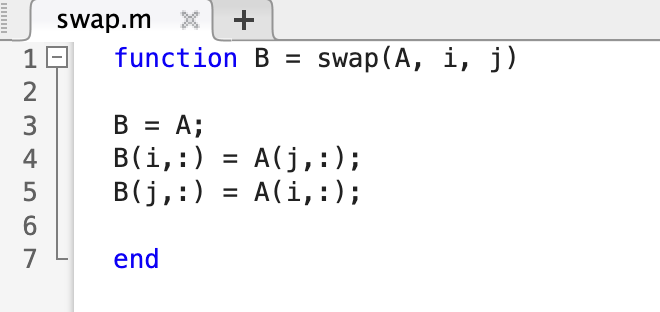
\includegraphics[scale=0.6]{swap.png}}
        \qquad\qquad$swap.m$\label{fig:1}
    \end{minipage}    
    \qquad\qquad\quad
    \begin{minipage}{.4\textwidth}
        \centering
        {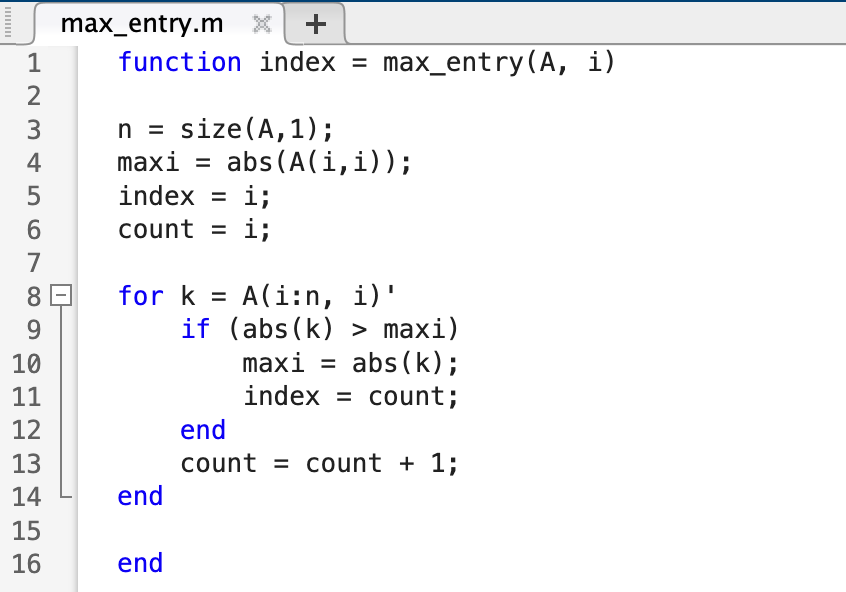
\includegraphics[scale=0.45]{max_entry.png}}
        \qquad\qquad$max\_entry.m$\label{fig:2}
    \end{minipage}        
\end{figure} 

\end{document}